\documentclass[a4paper,8pt]{article}

\usepackage{parskip}
\usepackage{fontspec}
\usepackage{graphicx}
\usepackage[usenames,dvipsnames]{xcolor}
\usepackage[scale=0.9, top=.4in, bottom=.4in]{geometry}
\usepackage{array}
\usepackage{tabularx}
\usepackage{enumitem}
\usepackage{titlesec}
\usepackage{hyperref}
\usepackage{fontawesome5}
\usepackage[normalem]{ulem}
\usepackage[none]{hyphenat}

\sloppy

\newcolumntype{C}{>{\centering\arraybackslash}X}

\titleformat{\section}{\Large\scshape\raggedright}{}{0em}{}[\titlerule]
\titlespacing{\section}{0pt}{6pt}{4pt}

\setmainfont{Arial}
\setlength{\parskip}{3pt}

\begin{document}
\pagestyle{empty}

% ================= HEADER =================

\begin{tabularx}{\linewidth}{@{} X r @{}}

\begin{tabular}{@{}l@{}}
{\color[HTML]{1C033C}\Huge Souraj Pal}\\[4pt]

\textcolor[HTML]{371e77}{\faEnvelope\ paulsouraj99@gmail.com \quad
\faMobile\ +91-8583-944-249}\\[2pt]

\textcolor[HTML]{371e77}{
\faGithub\ \underline{https://github.com/cureius}
\quad
\faLinkedin\ \underline{https://www.linkedin.com/in/souraj-pal-a257371b4/}
}
\end{tabular}
&
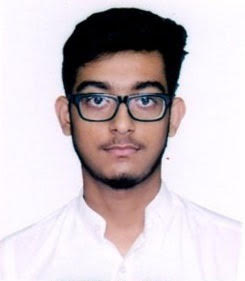
\includegraphics[width=1.8cm,height=2.2cm,keepaspectratio]{PIC.jpeg}

\end{tabularx}

% ================= SKILLS =================

\vspace{6pt}
\section{Skills}

\textbf{Languages:} Java, Kotlin, TypeScript, JavaScript, Dart\\
\textbf{Backend \& Platform:} Quarkus, Node.js, Express, REST, GraphQL, Kafka, MongoDB, Microservices, Multi-tenant Architecture\\
\textbf{Mobile \& Frontend:} Android, React Native, Flutter, ReactJS, NextJS\\
\textbf{Cloud \& DevOps:} AWS (EC2, S3), Docker, CI/CD, Nginx, GitHub Actions

% ================= WORK EXPERIENCE =================

\section{Work Experience}

% -------- Finfactor --------
\begin{tabularx}{\linewidth}{@{} X r @{}}
\textbf{Finfactor Technologies Pvt Ltd, Pune} & \color[HTML]{371e77} April 2025 -- Present\\
\textit{\textbf{Senior Software Engineer}} &
\end{tabularx}

\begin{itemize}[leftmargin=2em,itemsep=4pt]
\item Architected multi-tenant \textbf{PDF parser micro-services} to convert bank statements into \textbf{account-aggregator (ReBIT) compliant data} using \textbf{Quarkus} and \textbf{React}, improving onboarding throughput by \textbf{85\%}.
\item Built backend services for \textbf{bank statement analysis} deriving \textbf{loan eligibility scores} and \textbf{sector-wise income and expenditure models} for \textbf{salaried users and SMEs}.
\item Developed an \textbf{Early Warning Signals (EWS)} platform using \textbf{expenditure trends} and \textbf{category-wise behaviour analysis} to generate \textbf{real-time risk alerts} and portfolio insights.
\item Built a role-based \textbf{web dashboard} and \textbf{React Native mobile app} for lender risk analysis and borrower monitoring.
\item Delivered a \textbf{multi-tenant underwriting and monitoring platform} with \textbf{AA consent management} and \textbf{analytics visualisation} for financial institutions.
\end{itemize}

\vspace{6pt}

% -------- GoDeskless --------
\begin{tabularx}{\linewidth}{@{} X r @{}}
\textbf{GoDeskless Inc, Pune} & \color[HTML]{371e77} Jan 2022 -- April 2025\\
\textit{\textbf{Software Engineer}} &
\end{tabularx}

\begin{itemize}[leftmargin=2em,itemsep=4pt]
\item Built multiple \textbf{Android applications} including \textbf{Field Service}, \textbf{CRM} and \textbf{Lead Management} platforms using \textbf{Kotlin}, \textbf{Java}, \textbf{MVVM} and \textbf{Clean Architecture}.
\item Implemented \textbf{live tracking}, \textbf{geofencing}, \textbf{geotagging}, \textbf{video calling} and \textbf{chat} features using \textbf{Google Maps}, \textbf{CouchDB} and \textbf{WebSockets}, increasing customer acquisition by \textbf{66\%}.
\item Developed backend services with \textbf{Node.js}, \textbf{Express}, \textbf{REST}, \textbf{GraphQL}, \textbf{SSE} and \textbf{Socket APIs}.
\item Built a \textbf{React Native} and \textbf{native Android} contact-centre solution integrated with \textbf{Salesforce}.
\item Delivered cross-platform mobile applications using \textbf{Flutter} and native bridges; integrated video calling using \textbf{OpenTok}, improving ticket closure by \textbf{50\%}.
\item Worked on \textbf{AWS (S3, EC2, CloudFront)}, \textbf{Docker}, \textbf{Portainer}, \textbf{Nginx}, \textbf{Cloudflare} and \textbf{GitHub Actions} for CI/CD, reducing operational dependency by \textbf{33\%}.
\end{itemize}

\vspace{6pt}

% -------- Archies Intern --------
\begin{tabularx}{\linewidth}{@{} X r @{}}
\textbf{Archies InfoTech, Kolkata} & \color[HTML]{371e77} Aug 2021 -- Jan 2022\\
\textit{\textbf{Software Engineering Intern}} &
\end{tabularx}

\begin{itemize}[leftmargin=2em,itemsep=4pt]
\item Built peer-to-peer \textbf{chat} and \textbf{video communication} applications using \textbf{native Android} and \textbf{MongoDB}.
\item Integrated real-time audio and video conferencing using \textbf{Agora SDK}.
\item Developed a full-stack \textbf{e-commerce platform} with \textbf{Android}, \textbf{ReactJS}, \textbf{Redux} and \textbf{Express}.
\item Contributed to \textbf{location-based matching} and \textbf{cab-booking applications} using \textbf{Google Maps} and location APIs.
\end{itemize}

% ================= EDUCATION =================

\vspace{6pt}
\section{Education}

\begin{tabularx}{\linewidth}{@{} X r @{}}
\textbf{RCC Institute of Information Technology} & \color[HTML]{371e77} Jul 2019 -- Jun 2023\\
Bachelor of Technology (Electronics and Communication Engineering) & \textbf{CGPA: 8.94/10}\\[6pt]

\textbf{Narendranath Vidyamandir} & \color[HTML]{371e77} Jul 2017 -- Jun 2019\\
Higher Secondary (Science) & \textbf{CGPA: 8.22/10}\\[6pt]

\textbf{Barrackpore Ramakrishna Vivekananda Mission} & \color[HTML]{371e77} Jan 2006 -- Jun 2017\\
Secondary Education (WBBSE) & \textbf{CGPA: 8.77/10}
\end{tabularx}

% Projects
\section{Personal Projects} \begin{tabularx}{\linewidth}{ @{}l r@{} } \begin{minipage}[t]{\linewidth} \begin{itemize}[nosep,after=\strut, leftmargin=2em, itemsep=2pt] \item \textbf{FoodGrid (01/2026 - 02/2026):} Modern POS and Management For Modern Restaurants. which has \textbf{QR Ordering}, \textbf{Smart KOT System}, \textbf{Analytics}, \textbf{Multi-Outlet support}, \textbf{Swiggy and Zomato integration}, \textbf{Payment Gateway integration}\href{https://github.com/cureius/FoodGrid}{\textcolor[HTML]{371e77}{FoodGrid}}. Used \textbf{Quarkus} in backend and \textbf{NextJs} for frontend , integrated payments with \textbf{Rezorpay}. \item \textbf{Pathshala-app (04/2020 - 07/2020):} Online \textbf{Education} \textbf{platform} \textbf{(Native Android)} for the needy students, which gives liberty to the teachers to be independent about their Brand(s) and fees. It has all the pros of every Ed-tech app in the market, without including their single cons.\href{https://github.com/cureius/pathshala-app}{\textcolor[HTML]{371e77}{Pathshala-App}}. Used \textbf{MVVM} Architecture and integrated \textbf{UPI}. \item \textbf{Drive-Safe (09/2020 - 10/2020):} If any accident occurs, this app will automatically send \textbf{SOS} and the location of nearest \textbf{Hospitals} and \textbf{Police Station} to the family and friends (pre-enrolled) of the victim. Used \textbf{Arduino} \& \textbf{Gyroscope}. \item \textbf{Pocket (01/2023 - 04/2023):} A sophisticated expense tracking and money management application. Which automatically detects transactions from SMS, and also categorize the transaction depending on the narration and transaction details. Built with \textbf{Kotlin}, \textbf{Jetpack-Compose} \& implements \textbf{Clean Architecture}. \end{itemize} \end{minipage} \end{tabularx} 
% Leadership and Volunteering 
\section{Freelancing Experience} \begin{tabularx}{\linewidth}{ @{}l r@{} } \begin{minipage}[t]{\linewidth} \begin{itemize}[nosep,after=\strut, leftmargin=2em, itemsep=2pt] \item \textbf{FitMedik (09/2021 - 01/2022):} App (along with tracker band) to track the vitals of the doctors and health-care persons to notify them of their health conditions. Used React Native and \textbf{BLE(Bluetooth Low Energy)} for data fetching. \item \textbf{StreamLiner (08/2024 - 11/2024):} Developed a Total \textbf{Inventory and Employee Management System} , Which automats the \textbf{Vendor , Customer billing} and \textbf{employee salary}. Automated \textbf{PDF invoice generation} and email notification. With the help of this, the operation efficiency will increase by \textbf{80\%}.
% Leadership and Volunteering 
\section{Achievements} \begin{tabularx}{\linewidth}{ @{}l r@{} } \begin{minipage}[t]{\linewidth} \begin{itemize}[nosep,after=\strut, leftmargin=2em, itemsep=2pt] \item \textbf{Best Performer Award:} Honored with Best Performer Award (3ed Quater 2022 + 4th Quater 2023). \item \textbf{Smart India Hackathon (SIH-2022):} Finalist of Smart India Hackathon (SIH-2022). Developed a healthcare application and integrated voice commands as well. \item \textbf{Domain Head (Android):} Head of the \textbf{Android Development Club} in college and conducted multiple workshops. \end{itemize} \end{minipage} \end{tabularx} \end{document}

\end{document}